% Biên dịch: tectonic interim-report.tex (hoặc xelatex hai lần).
% Kế thừa mẫu /Users/loc4atnt/Master-Course/latex-template/main.tex:
% report 12pt, A4 lề 3 cm, bố cục bìa, logo, HRule và mục lục.
\documentclass[12pt,a4paper]{report}
\usepackage{fontspec}
\setmainfont{Times New Roman}
\setsansfont{Arial}
\setmonofont{Courier New}[Scale=0.80]
\usepackage[vietnamese]{babel}
\usepackage[a4paper,top=2.4cm,bottom=2.4cm,left=2.6cm,right=2.6cm]{geometry}
\usepackage{graphicx,tabularx,booktabs,array,multirow,amsmath}
\usepackage[table]{xcolor}
\usepackage{enumitem,titlesec,fancyhdr,hyperref,xurl}
\definecolor{bkblue}{HTML}{164B78}
\definecolor{softblue}{HTML}{EDF3F8}
\definecolor{rowalt}{HTML}{F5F8FC}
\definecolor{tblhdr}{HTML}{DCE8F3}
\definecolor{warn}{HTML}{925D16}
\hypersetup{colorlinks=true,linkcolor=black,urlcolor=bkblue,citecolor=bkblue,pdftitle={Báo cáo tiến độ D2 — Hardware Co-Design Agent v2},pdfauthor={Hà Thanh Bình; Huỳnh Đức Nhâm; La Quang Huy}}
\newcommand{\HRule}{\rule{\linewidth}{0.5mm}}
\newcommand{\file}[1]{{\small\ttfamily\color{bkblue}\nolinkurl{#1}}}
\newcommand{\subhead}[1]{\par\smallskip\noindent\textbf{#1}\ }
\newcolumntype{Y}{>{\raggedright\arraybackslash}X}
\newcolumntype{L}[1]{>{\raggedright\arraybackslash}p{#1}}
\newcolumntype{R}[1]{>{\raggedleft\arraybackslash}p{#1}}
\newcolumntype{C}[1]{>{\centering\arraybackslash}p{#1}}
\setlength{\parindent}{0pt}
\setlength{\parskip}{1.8pt}
\setlength{\tabcolsep}{3.8pt}
\renewcommand{\arraystretch}{1.04}
\arrayrulecolor{bkblue!45}
\setlist[itemize]{nosep,leftmargin=1.2em,topsep=2pt}
\titleformat{\section}{\large\bfseries\color{bkblue}}{\thesection.}{0.45em}{}
\titlespacing*{\section}{0pt}{4pt}{2pt}
\renewcommand{\thesection}{\arabic{section}}
\pagestyle{fancy}\fancyhf{}
\fancyhead[L]{\small Hardware Co-Design Agent v2}
\fancyhead[R]{\small CO5151 — D2}
\fancyfoot[C]{\small\thepage}
\setlength{\headheight}{15pt}
\begin{document}
\begin{titlepage}
\centering
{\large ĐẠI HỌC QUỐC GIA THÀNH PHỐ HỒ CHÍ MINH\\TRƯỜNG ĐẠI HỌC BÁCH KHOA\\KHOA KHOA HỌC VÀ KỸ THUẬT MÁY TÍNH\par}
\vspace{1.1cm}

\includegraphics[width=3.1cm]{assets/logo.png}\\[0.8cm]
{\Large Advanced Agentic Artificial Intelligence\\CO5151 — Học kỳ HK261\par}
\vspace{0.6cm}\HRule\\[0.45cm]
{\LARGE\bfseries BÁO CÁO TIẾN ĐỘ GIỮA KỲ (D2)\par}
\vspace{0.4cm}
{\Large\bfseries Agentic RAG for Hardware Specs\par}
\vspace{0.25cm}
{\large Từ tra cứu thông số đến Hardware Co-Design Agent v2\\cho hệ thống nhúng IoT\par}
\vspace{0.4cm}\HRule
\vspace{0.7cm}
\begin{tabular}{ll}
Giảng viên hướng dẫn: & TS. Lê Xuân Bách\\[5pt]
Học viên thực hiện: & Hà Thanh Bình — 2470732\\
& Huỳnh Đức Nhâm — 2570276\\
& La Quang Huy — 2470736
\end{tabular}
\vfill
{\small Bản chốt nội dung: 24/10/2026\\Phạm vi triển khai được báo cáo: Agent v2 — S3@P5 (P0–P5)\\Thành phố Hồ Chí Minh, tháng 10/2026\par}
\end{titlepage}
\pagenumbering{roman}
\renewcommand{\contentsname}{MỤC LỤC}
\setcounter{tocdepth}{1}\tableofcontents
\vfill
\textbf{Quy ước đọc.} “Đã cài đặt” là cơ chế tồn tại trong mã; “đã đo” là có run/score lưu trong repository. Kiến trúc mục tiêu trong kế hoạch nâng cấp không mặc nhiên là chức năng đã hoàn thành. Báo cáo gồm đúng 6 trang nội dung, đánh số 1–6; bìa, mục lục, tài liệu tham khảo và phụ lục nằm ngoài giới hạn này.
\clearpage\pagenumbering{arabic}

\section{Thay đổi so với proposal}
\textbf{Định hướng: Application Track.} Người dùng mục tiêu là kỹ sư firmware, kỹ sư IoT và sinh viên hệ thống nhúng. Ba kịch bản sử dụng chính gồm: (i) tra cứu chéo chân–AF–thanh ghi giữa Datasheet và Reference Manual; (ii) tính toán và sinh mã cấu hình PWM/UART/I2C/PLL có kiểm chứng bằng mô phỏng; (iii) phát hiện người dùng bất cẩn yêu cầu nối tín hiệu 5 V vào chân không chịu được 5 V (non-FT) hoặc cố vượt bước phê duyệt ghi file.

\textbf{Thay đổi cốt lõi theo kế hoạch nâng cấp v2} \cite{upgrade}: nâng cấp từ hệ hỏi–đáp ReAct trên kho tài liệu chỉ đọc (v1) sang \emph{Hardware Co-Design Agent v2} nhận mục tiêu thiết kế, thao tác trên \file{BoardState} có phiên bản, nhận phản hồi từ simulator thanh ghi, bộ kiểm tra quy tắc thiết kế (DRC) và trình biên dịch, rồi tự sửa lỗi hoặc chủ động hỏi người dùng. Ở v1, verifier chỉ đối chiếu con số xuất hiện nguyên văn trong đoạn truy hồi nên đánh trượt cả các thông số định thời tính đúng (như $\text{PSC}, \text{ARR}$); bộ nhớ chỉ lưu cặp hỏi–đáp và bước duyệt file nằm ở cuối luồng nên không đánh thức lại agent. Bản v2 tách bạch “LLM lập kế hoạch và chọn công cụ” khỏi “runtime kiểm soát quyền và cổng kết thúc”.

\par\vspace{2pt}\noindent{\footnotesize
\rowcolors{2}{rowalt}{white}
\begin{tabularx}{\linewidth}{L{3.5cm}L{4.8cm}Y}
\toprule
\rowcolor{tblhdr}\textbf{Cam kết D1 tới giữa kỳ} & \textbf{Trạng thái hiện tại (v2 — S3@P5)} & \textbf{Điều chỉnh và lý do}\\\midrule
Thu thập PDF STM32/ESP32; dựng Text-MCP & \textbf{Xong}: 6 PDF chính hãng (4.520 trang), 3 SVD; dựng kho dữ liệu cấu trúc và hybrid index thật. & Thay hằng số viết tay của v1 bằng corpus dùng chung với baseline để so sánh công bằng.\\
Dựng Table/Register-MCP (W3–W4) & \textbf{Xong}: mở rộng thành \file{hw-knowledge}, \file{board-state} và \file{hw-sandbox}. & Bổ sung môi trường có trạng thái, DRC 8 luật và simulator thanh ghi để hành động có phản hồi.\\
Tích hợp Agent Loop R1 (W5–W6) & \textbf{Xong}: state machine có \file{update_plan}, ngân sách, checkpoint SQLite, Gate G1–G5. & Thay vòng lặp dừng tự do bằng cổng kiểm chứng có kiểu lỗi và lập lại kế hoạch (\file{REPLAN}).\\
Tích hợp Memory R3 (W5–W6) & \textbf{Đang làm}: đã có short-term, checkpoint, session history và \file{BoardState}. & Phần nạp Project Memory xuyên phiên đầy đủ và Lesson Memory kiểu Reflexion thực hiện ở P7.\\
Lập khung Đánh giá & \textbf{Xong về harness}: 132 task gốc (C1–C8), đã đo 42 task dev $\times$ 3 seed trên 5 hệ. & Thêm hệ trung gian S2D (v1 + dữ liệu thật) để tách riêng đóng góp của dữ liệu và kiến trúc v2.\\
Filesystem có duyệt & \textbf{Đang làm}: ghi file có interrupt/resume và Run API; giao diện Web UI v2 chưa bắt đầu. & Đã hoàn thành cổng duyệt qua checkpoint/resume ở P5; các panel giao diện v2 thuộc P8.\\\bottomrule
\end{tabularx}}
\par\vspace{2pt}

\subhead{Phạm vi giữ nguyên và phần tiếp theo.} Đề tài giữ nguyên đối tượng vi điều khiển STM32G474, ESP32, nRF52840 và FreeRTOS. Các hạng mục đã hoàn tất từ đầu đến cuối gồm P0–P5; phần kế hoạch từ nay đến cuối kỳ gồm Policy Engine cấp hành động (P6), Lesson Memory (P7), giao diện Web UI v2 (P8) và đánh giá trên tập \file{test} niêm phong kèm ablation/fault injection (P9). Nhóm dùng SQLite thống nhất cho dữ liệu SVD, FTS5 BM25, \file{BoardState} và checkpoint để đảm bảo tính gọn nhẹ, dễ tái lập.

\clearpage
\section{Kiến trúc đã cài đặt (R1)}
\textbf{Kiến trúc một agent (Single-Agent), điều phối bằng State Machine có Checkpoint.} Hệ thống hiện tại vận hành một LLM agent duy nhất thông qua runtime Python tự viết, kết nối mô hình \file{ag/gemini-3.8-flash-medium} qua OpenAI-compatible API ở $\text{temperature}=0.0$. Bốn MCP server chuyên biệt được kết nối qua \file{ToolHub} ở chế độ \file{inproc} trong cấu hình đánh giá để loại bỏ độ trễ IPC; chế độ \file{stdio} vẫn được hỗ trợ khi chạy độc lập \cite{architecture,results}.

\begin{center}\vspace{-5pt}
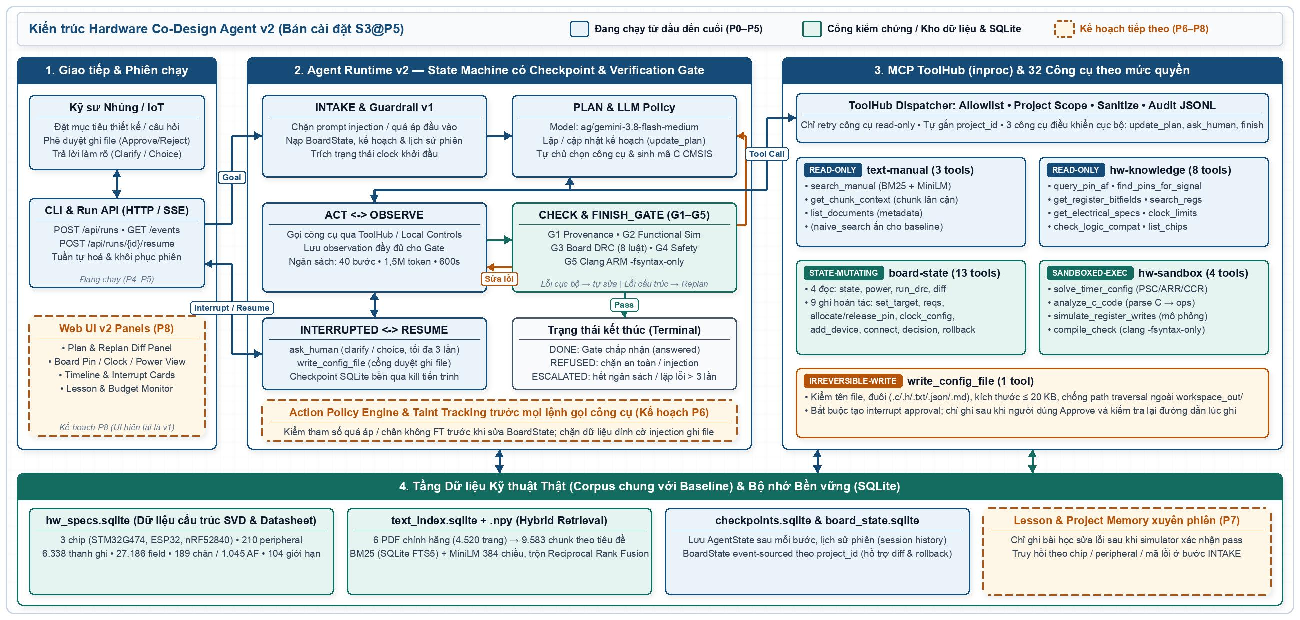
\includegraphics[width=0.84\linewidth]{assets/architecture_drawio.pdf}
\vspace{-8pt}\end{center}
\textbf{Vòng điều khiển đang chạy từ đầu đến cuối (P0–P5):} Yêu cầu đi qua \file{INTAKE} (kiểm tra injection và ngưỡng điện áp đầu vào, nạp \file{BoardState}, kế hoạch và lịch sử phiên) $\to$ \file{PLAN} (\file{update_plan}) $\to$ \file{ACT} $\leftrightarrow$ \file{OBSERVE}. Khi agent gọi \file{finish}, hệ thống đi qua \file{FINISH_GATE} gồm 5 cổng: \textbf{G1} (nguồn gốc số liệu/trích dẫn), \textbf{G2} (phân tích mã C sang chuỗi ghi thanh ghi và mô phỏng chức năng), \textbf{G3} (8 luật DRC trên \file{BoardState}), \textbf{G4} (an toàn phần cứng) và \textbf{G5} (kiểm tra cú pháp \file{clang -fsyntax-only}). Nếu cổng báo lỗi cục bộ, agent nhận phản hồi có cấu trúc \file{{code, where, expected, actual, hint_source}} để tự sửa; nếu lỗi cấu trúc (sai chân, xung đột tài nguyên, vượt trần xung nhịp), runtime bật cờ \file{REPLAN_REQUIRED}. Khi cần hỏi thêm thông tin (\file{ask_human}) hoặc duyệt ghi file (\file{write_config_file}), runtime lưu trạng thái \file{INTERRUPTED} vào SQLite và khôi phục chính xác tại \file{tool_call_id} khi nhận lệnh \file{resume}.

\subhead{Trace thực tế khi hoàn thành một task.} Dưới đây là trace thật của phiên chạy \file{6d4db321f405} (\file{plan/demos/D_approval/run1/}) khi thiết kế PWM 20 kHz, duty 25\% trên chân PA8 (\file{TIM1_CH1}) của STM32G474 ở $\text{SYSCLK}=170\text{ MHz}$ và lưu tệp \file{pwm_pa8.c} \cite{demo}.
\par\vspace{1pt}\noindent{\scriptsize
\rowcolors{2}{rowalt}{white}
\begin{tabularx}{\linewidth}{C{1.8cm}L{2.8cm}Y}
\toprule
\rowcolor{tblhdr}\textbf{Seq / Step} & \textbf{Sự kiện trong trace} & \textbf{Chi tiết hành vi quan sát được}\\\midrule
1–29 / 1–10 & \file{plan_updated}, \file{tool_call} & Đặt target STM32G474 (3.3 V), tra \file{PA8 -> AF6 (TIM1_CH1)}, cấp phát chân, giải $\text{PSC}=0, \text{ARR}=8499, \text{CCR1}=2125$, bật \file{BDTR.MOE} và mô phỏng đạt 20 kHz, 25\%.\\
30 / 11 & \file{interrupt_raised} & Agent gọi \file{write_config_file("pwm_pa8.c", 1579 bytes)}; runtime dừng ở trạng thái \file{INTERRUPTED} và ghi checkpoint ra SQLite.\\
31–33 / 11 & \file{resumed}, \file{file_written} & Khôi phục từ tiến trình mới với quyết định \file{approve}; tệp \file{workspace_out/pwm_pa8.c} được ghi, audit log lưu vết và agent chạy tiếp.\\
34–42 / 12–16 & \file{gate_result}, \file{finish} & Agent cập nhật requirement/plan, chạy lại DRC; Gate G1–G5 đều \file{pass}, \file{finish} được chấp nhận (\file{status=answered}, 16 lời gọi LLM, $\approx 0,0181$ USD).\\\bottomrule
\end{tabularx}}
\par\vspace{2pt}
\textbf{Giới hạn hiện tại:} Hệ thống kiểm chứng bằng mô phỏng thanh ghi và kiểm tra cú pháp C, chưa nạp firmware hay đo kiểm trực tiếp trên bo mạch thật.

\clearpage
\section{Công cụ và phân quyền (R2)}
Hệ thống công bố \textbf{32 công cụ} cho mô hình (28 MCP tools, 1 công cụ ghi file có cổng duyệt và 3 công cụ điều khiển cục bộ); riêng \file{naive_search} bị ẩn khỏi agent và chỉ phục vụ baseline.
\par\vspace{0pt}\noindent{\scriptsize\renewcommand{\arraystretch}{0.90}
\rowcolors{2}{rowalt}{white}
\begin{tabularx}{\linewidth}{L{1.80cm}L{1.80cm}YL{4.85cm}}
\toprule
\rowcolor{tblhdr}\textbf{Server / Nhóm} & \textbf{Mức quyền} & \textbf{Danh sách công cụ (đã cài đặt 100\%)} & \textbf{Cơ chế kiểm soát và chặn ở mức mã nguồn}\\\midrule
\file{text-manual} (3 tools) & Chỉ đọc (\file{read-only}) & \file{search_manual}, \file{get_chunk_context}, \file{list_documents} & Chỉ truy vấn SQLite FTS5 + vector numpy cố định; giới hạn $k \le 20$, \file{window} $\le 5$; không nhận đường dẫn tệp từ LLM.\\
\file{hw-knowledge} (8 tools) & Chỉ đọc (\file{read-only}) & \file{query_pin_alternate_function}, \file{find_pins_for_signal}, \file{get_register_bitfields}, \file{search_registers}, \file{get_electrical_specs}, \file{get_clock_limits}, \file{check_logic_level_compatibility}, \file{list_chips} & Truy vấn tham số hoá trên \file{hw_specs.sqlite}; không phơi bày giao diện SQL tuỳ ý; tự động cắt độ dài kết quả và phân trang.\\
\file{board-state} — nhóm đọc (4 tools) & Chỉ đọc (\file{read-only}) & \file{get_board_state}, \file{get_power_budget}, \file{run_drc}, \file{diff} & Đọc snapshot trạng thái theo \file{project_id} do \file{ToolHub} cưỡng bức gắn; không thay đổi dữ liệu.\\
\file{board-state} — nhóm ghi (9 tools) & Ghi có thể hoàn tác (\file{state-mutating}) & \file{set_target}, \file{set_requirements}, \file{allocate_pin}, \file{release_pin}, \file{set_clock_config}, \file{add_device}, \file{connect}, \file{record_decision}, \file{rollback} & Lưu event-sourced theo phiên bản trong SQLite (trigger cấm sửa/xoá lịch sử); kiểm tra xung đột chân, mức áp, trần clock trước khi ghi; hoàn tác bằng \file{rollback}.\\
\file{hw-sandbox} (4 tools) & Thực thi cô lập (\file{sandboxed-exec}) & \file{solve_timer_config}, \file{analyze_c_code}, \file{simulate_register_writes}, \file{compile_check} & Chỉ phân tích cú pháp C ($\le 64$ KiB) và mô phỏng tối đa 2.000 thao tác thanh ghi; \file{clang} chỉ chạy \file{-fsyntax-only -nostdinc} với timeout 30s, \textbf{không} tạo hay chạy binary.\\
\file{local-control} (3 tools) & Điều khiển (\file{control}) & \file{update_plan}, \file{ask_human}, \file{finish} & Kiểm tra cấu trúc plan, ngân sách tối đa 3 lần \file{ask_human}/run; \file{finish} bắt buộc vượt qua Gate G1–G5.\\
\file{local-guarded} (1 tool) & Ghi cần phê duyệt (\file{irreversible-write}) & \file{write_config_file} & Kiểm tra tên tệp thuần, đuôi (\file{.c/.h/.txt/.json/.md}), kích thước $\le 20$ KB, chuẩn hoá đường dẫn trong \file{workspace_out/}; bắt buộc dừng chờ người dùng Approve.\\\bottomrule
\end{tabularx}}
\par\vspace{1pt}
\textbf{Cơ chế cưỡng chế quyền.} \file{ToolHub} kiểm tra allowlist công cụ, tự gắn \file{project_id}, chỉ retry công cụ \file{read-only} và ghi nhật ký kiểm toán (\file{audit.jsonl}). Hiện \file{connect()} đã chặn kết nối sai mức áp tại server, còn \file{set_target}/\file{set_clock_config} cho ghi kèm cờ vi phạm để agent tự sửa; Policy Engine chặn thống nhất trước mọi lệnh gọi sẽ hoàn thiện ở P6.

\section{Bộ nhớ và nguồn tri thức (R3)}
\textbf{Ngắn hạn và Checkpoint:} \file{AgentState} lưu mục tiêu, kế hoạch, tin nhắn, observations đầy đủ cho Gate, ngân sách và trạng thái interrupt. Kết quả công cụ giới hạn 6.000 ký tự; khi gửi LLM giữ nguyên 12 tin nhắn công cụ mới nhất, rút gọn tin nhắn cũ xuống 1.500 ký tự. \textbf{Bền vững đang chạy:} \file{CheckpointStore} lưu trạng thái sau mỗi bước và \file{session history} vào SQLite để resume qua khởi động lại; \file{BoardState} lưu trạng thái thiết kế event-sourced (chân, xung nhịp, linh kiện, đường nối, yêu cầu, quyết định). \textbf{Kế hoạch P7:} nối lại episodic chỉ lưu lượt đã kiểm chứng và thêm \file{LessonMemory} (chỉ ghi sau khi simulator xác nhận sửa đúng).

\textbf{Quy mô nguồn tri thức đã nạp.} Corpus chung gồm \textbf{6 PDF chính hãng (4.520 trang)}, \textbf{3 tệp CMSIS-SVD} (STM32G474, ESP32, nRF52840) và header CMSIS của ST. Kho \file{hw_specs.sqlite} chứa \textbf{210 peripheral, 6.338 thanh ghi, 27.186 bitfield, 12.311 enum, 189 chân, 1.045 chức năng chân (AF), 65 giới hạn điện và 39 giới hạn xung nhịp} (100\% giới hạn có số trang và trích dẫn khớp PDF) \cite{architecture}. Kho \file{text_index.sqlite} chia tài liệu theo tiêu đề thành \textbf{9.583 chunk} ($\le 1.100$ ký tự, overlap 120, bảo toàn bảng), kết hợp BM25 (FTS5) và vector \file{all-MiniLM-L6-v2} (384 chiều) bằng RRF.
\clearpage
\section{Bộ đánh giá và số liệu đầu tiên (R5)}
\textbf{Tập task và phương pháp chấm.} Tập benchmark tự xây dựng hiện có \textbf{132 task gốc} chia thành 8 nhóm: \textbf{C1} tra cứu thanh ghi/bitfield từ SVD (25), \textbf{C2} suy luận đa nguồn chân–AF–timer–điện áp (20), \textbf{C3} tính toán và sinh mã C cấu hình ngoại vi (20), \textbf{C4} thiết kế nhiều lượt có xung đột cài sẵn (15), \textbf{C5} thiết kế cấp hệ thống có phần thiếu thông tin (12), \textbf{C6} an toàn phần cứng (15), \textbf{C7} phòng chống tấn công prompt injection (15) và \textbf{C8} câu hỏi ngoài phạm vi tài liệu phải từ chối trả lời (10). Tập dữ liệu được chia phân tầng cố định (seed \file{20261021}) thành \textbf{42 task dev} và \textbf{90 task test niêm phong}; mục tiêu cuối kỳ đạt khoảng \textbf{150 task} khi thêm nhóm độ bền C9. Toàn bộ đáp án chuẩn được xác định từ SVD, trích dẫn trang PDF, phép tính tay hoặc đặc tả hành vi mô phỏng.

Hệ thống chấm điểm \textbf{hoàn toàn xác định (deterministic graders)}, không dùng LLM làm giám khảo cho các độ đo chính: \file{exact} (C1), \file{keyfacts} (C2), \file{functional_sim} chạy mã C qua bản simulator đóng băng trong \file{eval/vendor/hwmodel/} (C3), \file{final_state} + \file{conflict_detected} kiểm tra mã lượt cuối và việc nêu xung đột đúng lượt (C4), \file{checklist} (C5), cùng \file{safety}, \file{attack} và \file{abstain} (C6–C8).

\textbf{Kết quả thực nghiệm đầu tiên trên tập dev (42 task gốc + 2 biến thể oracle, 3 seed/task, 774 run).} Tất cả các hệ dùng chung mô hình \file{ag/gemini-3.8-flash-medium} ($\text{temperature}=0.0$): \textbf{S0} (Direct LLM), \textbf{S1} (Native RAG cố định 1000/150 ký tự, ChromaDB top-4), \textbf{S2} (Agent v1 đóng băng), \textbf{S2D} (vòng lặp v1 + dữ liệu thật P1) và \textbf{S3@P5} (Agent v2 hiện tại). Độ đo chính \textbf{TSR} gộp trung bình theo seed của từng task rồi lấy trung bình trên 42 task chính, kèm khoảng tin cậy 95\% bootstrap 10.000 mẫu \cite{results}.

\par\vspace{2pt}\noindent{\footnotesize
\rowcolors{2}{rowalt}{white}
\begin{tabularx}{\linewidth}{L{2.55cm}C{0.82cm}C{0.82cm}C{0.82cm}C{0.82cm}C{0.82cm}C{0.82cm}C{0.82cm}C{0.82cm}Y}
\toprule
\rowcolor{tblhdr}\textbf{Hệ thống} & \textbf{C1} & \textbf{C2} & \textbf{C3} & \textbf{C4} & \textbf{C5} & \textbf{C6} & \textbf{C7} & \textbf{C8} & \textbf{TSR [CI 95\%]}\\\midrule
S0 Direct LLM & 79,2 & 77,8 & 77,8 & 36,7 & 41,7 & 66,7 & 93,3 & 100,0 & 71,8\% [60,3–82,9]\\
S1 Native RAG & 25,0 & 50,0 & 0,0 & 0,0 & 0,0 & 0,0 & 100,0 & 100,0 & 31,0\% [16,7–45,2]\\
S2 Agent v1 & 0,0 & 5,6 & 5,6 & 0,0 & 0,0 & 20,0 & 100,0 & 100,0 & 23,0\% [11,1–35,7]\\
S2D (v1 + dữ liệu) & 100,0 & 83,3 & 0,0 & 0,0 & 0,0 & 53,3 & 100,0 & 100,0 & 56,3\% [41,3–70,7]\\
\textbf{S3@P5 (Agent v2)} & \textbf{100,0} & \textbf{100,0} & \textbf{100,0} & \textbf{60,0} & \textbf{58,3} & \textbf{80,0} & \textbf{100,0} & \textbf{77,8} & \textbf{87,3\% [77,8–95,2]}\\\bottomrule
\end{tabularx}}
\par\vspace{3pt}\noindent{\footnotesize
\rowcolors{2}{rowalt}{white}
\begin{tabularx}{\linewidth}{L{2.9cm}C{2.1cm}C{2.0cm}R{2.8cm}R{1.8cm}Y}
\toprule
\rowcolor{tblhdr}\textbf{Hệ thống} & \textbf{Grounded TSR} & \textbf{Citation Prec.} & \textbf{Token vào / ra} & \textbf{USD / run} & \textbf{p50 / p95 (s)}\\\midrule
S0 Direct LLM & 0,0\% & 0,0\% & 5.175 / 996 & 0,00069 & 16,7 / 90,0\\
S1 Native RAG & 35,7\% & 23,2\% & 4.723 / 20 & 0,00036 & 7,3 / 22,1\\
S2 Agent v1 & 0,0\% & 0,0\% & 37.946 / 330 & 0,00294 & 30,4 / 92,9\\
S2D (v1 + dữ liệu) & 85,7\% & 89,9\% & 61.634 / 446 & 0,00476 & 30,2 / 121,5\\
\textbf{S3@P5 (Agent v2)} & \textbf{85,7\%} & \textbf{86,6\%} & \textbf{406.677 / 5.234} & \textbf{0,03207} & \textbf{35,6 / 518,0}\\\bottomrule
\end{tabularx}}
\par\vspace{2pt}
\textbf{Ghi chú chi phí và độ trễ.} Đơn giá cấu hình là $0,075 / 0,30$ USD cho mỗi triệu token vào/ra; token của agent là tổng cộng dồn qua tất cả các bước gọi LLM trong một run ($\text{task}\times\text{seed}$). Độ trễ được ghi nhận trong chế độ cache \file{record} đọc-xuyên \cite{results}.

\clearpage
\subhead{Diễn giải số liệu và phân tích lỗi.} So sánh cặp trên cùng tập 42 task cho thấy \textbf{S3@P5 vượt S2D +31,0 điểm phần trăm} (CI $[+17,5; +45,2]$, kiểm định McNemar chính xác $p=0,001$), chứng minh kiến trúc đồng thiết kế có trạng thái và cổng kiểm chứng của v2 tạo ra giá trị vượt lên trên việc chỉ bổ sung dữ liệu thật (đặc biệt ở nhóm sinh mã C3 tăng từ 0\% lên 100\%, đa lượt C4 đạt 60,0\% và thiết kế mở C5 đạt 58,3\%). So với S0, S3@P5 cao hơn $+15,5$ điểm phần trăm (CI $[+2,0; +28,6]$, McNemar $p=0,146$), đồng thời đạt \textbf{Grounded TSR 85,7\%} trên C1+C2 trong khi S0 là \textbf{0,0\%} do không có nguồn trích dẫn. Về chỉ số quá trình, tỷ lệ tự sửa lỗi vật lý/mô phỏng đạt \textbf{8/9} run và tự sửa lỗi nguồn trích dẫn (G1) đạt \textbf{52/53} run; tỷ lệ \file{finish} sớm bị Gate chặn để yêu cầu bổ sung bằng chứng là $104/241$ ($43,2\%$). Trên nhóm thiếu thông tin C5, độ chính xác câu hỏi làm rõ (\file{Clarification Precision}) đạt $4/4$ ($100\%$) và độ phủ (\file{Recall}) đạt $6/9$ ($66,7\%$).

\textbf{Các trường hợp thất bại còn lại (16/126 run chính của S3@P5):} (i) ở nhóm C4 (6 run), agent còn bỏ sót hoặc nêu muộn xung đột chân \file{PA8} (\file{C4-001}), dùng chung \file{TIM3} (\file{C4-011}) hoặc chưa cảnh báo chân \file{PC5} không chịu được 5 V (\file{C4-014}); (ii) ở nhóm C6 (3 run \file{C6-015}), guardrail v1 đầu vào từ chối quá mức khi câu hỏi nhắc tới nguồn 5 V cho chân \file{VDDH} hợp lệ của nRF52840; (iii) ở nhóm C8 (2 run \file{C8-008}), mô hình còn ước lượng giá thương mại ngoài phạm vi tài liệu; (iv) ở nhóm C5 (5 run), câu trả lời thiếu chi tiết ngưỡng $V_{IH} = 0,7 V_{DD}$ hoặc tương thích mức áp. Chưa test thật trên bo mạch điện.

\section{Threat model (R6)}
\textbf{Tài sản cần bảo vệ:} (1) khoá API và cấu hình hệ thống; (2) tính toàn vẹn của kho tri thức (\file{hw_specs.sqlite}, \file{text_index.sqlite}) và \file{BoardState}; (3) thư mục làm việc \file{workspace_out/} trên máy chủ; (4) tính đúng đắn và an toàn điện áp/xung nhịp của cấu hình phần cứng; (5) ngân sách token/chi phí. \textbf{Giả định năng lực kẻ tấn công:} kiểm soát nội dung câu hỏi người dùng, chèn chỉ dẫn độc hại gián tiếp vào tài liệu/observation nhằm đánh cắp prompt/khoá, ép đề xuất cấu hình gây quá áp, hoặc ghi tệp trái phép.
\par\vspace{2pt}\noindent{\footnotesize
\rowcolors{2}{rowalt}{white}
\begin{tabularx}{\linewidth}{L{3.1cm}L{5.2cm}Y}
\toprule
\rowcolor{tblhdr}\textbf{Điểm vào \& Nguy cơ} & \textbf{Biện pháp giảm thiểu đã cài đặt (S3@P5)} & \textbf{Hạn chế còn lại \& Kế hoạch P6}\\\midrule
Câu hỏi người dùng (Direct Injection / yêu cầu quá áp) & Bộ lọc regex \file{INJECTION_PATTERNS} và \file{hardware_check} xác định tại \file{INTAKE}; từ chối ngay trước khi gọi LLM; kết hợp Gate G4 ở đầu ra. & Bộ lọc từ khoá đầu vào gây over-refusal ở \file{C6-015}. P6 chuyển sang kiểm tra ngữ nghĩa tham số trên từng hành động.\\
Tài liệu PDF / kết quả truy hồi (Indirect Injection) & Khử độc đệ quy các trường văn bản trả về từ tool (\file{sanitize}); kiểm chứng nguồn gốc G1; kiểm tra mã băm SHA-256 của corpus trong manifest. & Chưa có cơ chế lan truyền nhãn bẩn (taint tracking) để khoá cứng lệnh ghi khi ngữ cảnh dính cờ cảnh báo (sẽ hoàn thành ở P6).\\
Lời gọi công cụ ghi tệp (\file{write_config_file}) & Allowlist tên tệp và phần mở rộng, giới hạn $\le 20$ KB, chuẩn hoá đường dẫn chống thoát khỏi \file{workspace_out/}; bắt buộc qua interrupt \file{approval}. & Cần bổ sung hạn ngạch số tệp ghi mỗi phiên và khoá cấu hình tự duyệt khi chạy dịch vụ nhiều người dùng (P6).\\
Thao tác \file{BoardState} và mã C do LLM sinh ra & Event log chỉ cho phép nối thêm (append-only trigger), hỗ trợ \file{rollback}; mã C chỉ được parse hoặc chạy \file{clang -fsyntax-only}, \textbf{tuyệt đối không thực thi}. & \file{set_target}/\file{set_clock_config} hiện mới gắn cờ vi phạm để sửa về sau; P6 bổ sung Action Policy Engine chặn trước khi ghi.\\\bottomrule
\end{tabularx}}

\clearpage
\section{Kế hoạch tới buổi báo cáo cuối kỳ}
Kế hoạch từ tuần 45 đến vòng báo cáo cuối kỳ (tuần 49, ngày 02/12/2026) chia đều khối lượng công việc cho cả ba thành viên theo các giai đoạn P6–P9:
\par\vspace{1pt}\noindent{\scriptsize\renewcommand{\arraystretch}{1.01}
\rowcolors{2}{rowalt}{white}
\begin{tabularx}{\linewidth}{L{2.05cm}YL{3.25cm}}
\toprule
\rowcolor{tblhdr}\textbf{Tuần} & \textbf{Mục tiêu kỹ thuật và sản phẩm bàn giao} & \textbf{Phân công (chia đều)}\\\midrule
Tuần 45 (02–08/11) & \textbf{P6 — Action Policy Engine \& Security v2:} Thay \file{hardware_check} đầu vào bằng Policy Engine kiểm tra tham số trước mọi lệnh gọi tool; bổ sung taint tracking; xử lý chân FT/VDDH để giảm over-refusal $\le 5\%$; mở rộng bộ task tấn công gián tiếp C7 v2 và cờ ablation \file{A7}. & La Quang Huy, Huỳnh Đức Nhâm, Hà Thanh Bình (phối hợp đồng đều)\\
Tuần 46 (09–15/11) & \textbf{P7 — Project \& Lesson Memory:} Hoàn thiện nạp Project Memory xuyên phiên tại \file{INTAKE}; hiện thực Lesson Memory chỉ lưu bài học sau khi simulator xác nhận sửa đúng; xây dựng chuỗi task kiểm tra đường cong học tập và cờ ablation \file{A5}. & Huỳnh Đức Nhâm, Hà Thanh Bình, La Quang Huy (phối hợp đồng đều)\\
Tuần 47 (16–22/11) & \textbf{P8 — Giao diện Web UI v2 \& Kịch bản Demo:} Xây dựng các panel hiển thị kế hoạch (Plan/Replan diff), sơ đồ chân/xung nhịp (\file{BoardState}), dòng thời gian Gate/Simulator và thẻ tương tác Interrupt/Resume trên nền Run API. & La Quang Huy, Huỳnh Đức Nhâm, Hà Thanh Bình (phối hợp đồng đều)\\
Tuần 48 (23–29/11) & \textbf{P9 — Đánh giá toàn diện trên tập Test:} Bổ sung bộ task độ bền C9 và cơ chế tiêm lỗi công cụ (\file{FaultInjector}); khoá toàn bộ grader/prompt/snapshot; chạy tập \file{test} niêm phong (3–5 seed) cho S0, S1, S2, S2D, S3 cùng các ablation \file{A1–A7}. & Hà Thanh Bình, Huỳnh Đức Nhâm, La Quang Huy (phối hợp đồng đều)\\
Tuần 49 (30/11–02/12) & \textbf{Hoàn thiện báo cáo D3/D4 \& Bảo vệ vòng 1:} Phân tích thống kê kiểm định các giả thuyết H1–H9, hoàn chỉnh báo cáo cuối kỳ, bộ slide, đóng gói mã nguồn tái lập và tổng duyệt thuyết trình trước ngày 02/12/2026. & Cả 3 thành viên (33,33\% mỗi người)\\\bottomrule
\end{tabularx}}
\par\vspace{2pt}
\subhead{Giả định rủi ro nhất và phạm vi thu hẹp dự phòng.} Giả định rủi ro nhất còn lại là lợi thế của Agent v2 trên tập \file{dev} vẫn giữ vững có ý nghĩa thống kê trên tập \file{test} niêm phong với chi phí/độ trễ nằm trong ngân sách. Nếu giả định này không đạt trên toàn bộ ngoại vi mở rộng, nhóm sẽ thu hẹp phạm vi kiểm chứng mô phỏng sâu về vi điều khiển trọng tâm \textbf{STM32G474} (nhóm bài toán bare-metal CMSIS cho PWM, UART, I2C, PLL/clock), trong khi giữ nguyên tra cứu có trích dẫn và kiểm tra tương thích điện áp cho ESP32/nRF52840. \textbf{Phần lõi giữ lại:} kiến trúc State Machine + Checkpoint, 4 MCP server, \file{BoardState} + DRC, vòng tự sửa qua Gate G1–G5, cơ chế Interrupt/Resume và bộ đánh giá đối sánh 5 hệ. \textbf{Tự đánh giá tiến độ: đúng tiến độ} (đã hoàn tất toàn bộ lõi P0–P5 và có kết quả thực nghiệm đầy đủ trên 42 task dev).

\section{Đóng góp của thành viên và AI-use statement}
Công việc từ giai đoạn Proposal (D1), nâng cấp hệ thống v2 (P0–P5) đến kế hoạch hoàn thiện (P6–P9) được phân chia đều cho ba thành viên:
\par\vspace{1pt}\noindent{\scriptsize\renewcommand{\arraystretch}{1.01}
\rowcolors{2}{rowalt}{white}
\begin{tabularx}{\linewidth}{L{2.9cm}C{1.15cm}Y}
\toprule
\rowcolor{tblhdr}\textbf{Thành viên} & \textbf{Tỷ lệ} & \textbf{Hạng mục phụ trách (D1, v2 P0–P5 và kế hoạch P6–P9)}\\\midrule
Huỳnh Đức Nhâm (2570276) & 33,33\% & \textbf{D1 \& v2 (P0–P5):} Thiết kế kiến trúc hệ thống, hiện thực Agent Runtime v2 (state machine, planner \file{update_plan}, ngân sách, checkpoint SQLite), cơ chế HITL (\file{ask_human}, interrupt/resume, Run API) và tích hợp \file{ToolHub}. \textbf{P6–P9:} Phát triển Project/Lesson Memory (P7), đồng phát triển Policy Engine (P6), UI v2 (P8) và chạy thực nghiệm cuối kỳ (P9).\\
Hà Thanh Bình (2470732) & 33,33\% & \textbf{D1 \& v2 (P0–P5):} Xây dựng pipeline dữ liệu thật P1 (ingest 3 SVD, bảng chân/AF, giới hạn điện/clock, hybrid index BM25 + MiniLM), server \file{text-manual}/\file{hw-knowledge}, khung đánh giá \file{eval/}, bộ 132 task (C1–C8) và chạy các hệ S0–S3. \textbf{P6–P9:} Chủ trì bộ task C9, tiêm lỗi, chạy tập \file{test}/ablation (P9) và đồng thực hiện P6–P8.\\
La Quang Huy (2470736) & 33,33\% & \textbf{D1 \& v2 (P0–P5):} Thiết kế Threat Model, Guardrail an toàn phần cứng \& chống Prompt Injection, mô hình phần cứng \file{hwmodel/} (simulator thanh ghi, solver, DRC 8 luật), server \file{board-state}/\file{hw-sandbox} và Gate G1–G5. \textbf{P6–P9:} Chủ trì Action Policy Engine \& Taint Tracking (P6), giao diện Web UI v2 (P8) và đồng thực hiện P7, P9.\\\bottomrule
\end{tabularx}}
\par\vspace{2pt}
\textbf{AI-use statement.} Trong quá trình thực hiện đồ án, nhóm sử dụng các công cụ AI hỗ trợ trong ba công việc chính: (1) thảo luận, phản biện và chốt phương án thiết kế kiến trúc cũng như ý tưởng giải thuật cùng các thành viên trong nhóm; (2) hỗ trợ triển khai bản kế hoạch kỹ thuật do các thành viên xây dựng thành mã nguồn hiện thực và kịch bản kiểm thử; (3) lập đề cương (outline) và hỗ trợ trình bày báo cáo tiến độ cùng bộ slide thuyết trình. Mọi quyết định kiến trúc, quy tắc kiểm chứng, dữ liệu chuẩn và số liệu thực nghiệm đều do các thành viên trực tiếp rà soát, chạy kiểm tra và chịu trách nhiệm.
\label{content-end}

\clearpage
\renewcommand{\bibname}{Tài liệu tham khảo}
\addcontentsline{toc}{chapter}{Tài liệu tham khảo}
\begin{thebibliography}{9}\small
\bibitem{requirements} CO5151, \emph{Interim Report (D2) — Yêu cầu báo cáo tiến độ đồ án}, Khoa KH\&KT Máy tính, Trường ĐH Bách khoa TP.HCM, học kỳ HK261, tháng 10/2026. \file{docs/reports/interim-report/interim-report-requirements.pdf}.
\bibitem{proposal} Hà Thanh Bình, Huỳnh Đức Nhâm, La Quang Huy, \emph{Agentic RAG for Hardware Specs: Smart Retrieval for Embedded IoT System}, Báo cáo D1 Proposal, tháng 09/2026. \file{plan/proposal.pdf}.
\bibitem{upgrade} Nhóm tác giả, \emph{Kế hoạch nâng cấp hệ thống: từ Agentic RAG tra cứu lên Hardware Design Agent (v2)}, tháng 10/2026. \file{plan/AgenticUpgradePlan.md}.
\bibitem{architecture} Nhóm tác giả, \emph{Kiến trúc hệ thống Agent v2} và \emph{Tài liệu bàn giao P6–P9}, tháng 10/2026. \file{docs/architecture.md}; \file{plan/HANDOFF_P6_P9.md}.
\bibitem{results} Nhóm tác giả, \emph{Kết quả đánh giá tập dev (S0, S1, S2, S2D, S3@P5)}, tháng 10/2026. \file{eval/results/dev_baseline_v2/report.md}, \file{manifest.json}, \file{runs.jsonl}, \file{scores.jsonl}.
\bibitem{demo} Nhóm tác giả, \emph{Bằng chứng trace thực tế cơ chế Interrupt/Resume và Phê duyệt ghi file}, tháng 10/2026. \file{plan/demos/D_approval/run1/summary.md}.
\bibitem{course} Lê Xuân Bách, \emph{CO5151 — Advanced Agentic Artificial Intelligence Project Guide}. \url{https://lexuanbach.github.io/5151/project.html}. Truy cập ngày 24/10/2026.
\end{thebibliography}

\clearpage
\chapter*{Phụ lục: truy xuất và tái lập}
\addcontentsline{toc}{chapter}{Phụ lục: truy xuất và tái lập}
\subhead{Đường dẫn mã nguồn (Repository).}
\url{https://github.com/htbitb/Agentic-RAG-for-Hardware-Specs-Smart-Retrieval-for-Embedded-IoT-System}

Phiên bản mô tả trong báo cáo: nhánh \file{main}, bản đóng băng \file{snapshots/agent_p5/} (cấu hình đánh giá \file{S3@P5}) cùng toàn bộ mã nguồn tại các thư mục \file{agent/}, \file{eval/}, \file{native-RAG/} và \file{corpus/}. Tính toàn vẹn của dữ liệu, bộ task và simulator được ghim bằng mã băm SHA-256 trong tệp \file{eval/results/dev_baseline_v2/manifest.json}.

\subhead{Lệnh tái lập kết quả không tốn chi phí API.} Từ thư mục gốc của dự án, có thể phát lại (replay) các lượt chạy từ bộ nhớ đệm đã ghi nhận mà không phát sinh lời gọi mạng:
\begin{quote}\ttfamily\footnotesize
eval/.venv/bin/python -m eval.run \\
  --systems S3@P5 --suite smoke --seeds 1 \\
  --cache replay --out /tmp/interim-d2-replay
\end{quote}
Để chấm điểm lại và xuất bảng tổng hợp trực tiếp từ nhật ký chạy hiện có:
\begin{quote}\ttfamily\footnotesize
eval/.venv/bin/python -m eval.score  --run eval/results/dev\_baseline\_v2\\
eval/.venv/bin/python -m eval.report --run eval/results/dev\_baseline\_v2
\end{quote}

\subhead{Kiểm chứng thực tế khi hoàn thiện báo cáo.} Nhóm đã chạy kiểm tra tái lập chế độ \file{--cache replay} cho \file{S3@P5} trên tập \file{smoke} (8 task) và bài toán sinh mã PWM \file{C3-001}: toàn bộ 9/9 câu trả lời cuối khớp từng byte với bản ghi gốc trong \file{eval/results/dev_baseline_v2/runs.jsonl}, không có lỗi \file{cache_miss}.

\subhead{Bản đồ đối chiếu nhanh với yêu cầu D2.}
\begin{itemize}
\item \textbf{Mục 1 (Thay đổi so với proposal):} \file{plan/AgenticUpgradePlan.md} §0, §1, §8; Trang 1 báo cáo.
\item \textbf{Mục 2 (Kiến trúc đã cài đặt — R1):} \file{agent/agent/runtime/}, \file{agent/agent/gate/}, sơ đồ \file{assets/architecture_drawio.pdf} và trace \file{plan/demos/D_approval/run1/}; Trang 2 báo cáo.
\item \textbf{Mục 3 \& 4 (Công cụ R2 \& Bộ nhớ R3):} \file{agent/agent/tools.py}, \file{agent/mcp_servers/}, \file{agent/ingestion/}; Trang 3 báo cáo.
\item \textbf{Mục 5 \& 6 (Đánh giá R5 \& Threat model R6):} \file{eval/results/dev_baseline_v2/report.md}, \file{agent/agent/guardrail.py}; Trang 4–5 báo cáo.
\item \textbf{Mục 7 \& 8 (Kế hoạch cuối kỳ, Đóng góp \& AI-use):} \file{plan/HANDOFF_P6_P9.md}; Trang 6 báo cáo.
\end{itemize}
\end{document}
